%%%%%%%%%%%%%%%%%%%%%%%%%%%%%%% beamer %%%%%%%%%%%%%%%%%%%%%%%%%%%%%%%%%%%%%%%%%%%%%%%%%
% To run - pdflatex filename.tex
%      acroread filename.pdf
%%%%%%%%%%%%%%%%%%%%%%%%%%%%%%%%%%%%%%%%%%%%%%%%%%%%%%%%%%%%%%%%%%%%%%%%%%%%%%%%%%%%%%%%

\documentclass[compress,oilve]{beamer}
\mode<presentation>

\usetheme[]{CambridgeUS}
% other themes: AnnArbor, Antibes, Bergen, Berkeley, Berlin, Boadilla, boxes, CambridgeUS, Copenhagen, Darmstadt, default, Dresden, Frankfurt, Goettingen,
% Hannover, Ilmenau, JuanLesPins, Luebeck, Madrid, Maloe, Marburg, Montpellier, PaloAlto, Pittsburg, Rochester, Singapore, Szeged, classic

\usecolortheme{beaver}
% color themes: albatross, beaver, beetle, crane, default, dolphin,  fly, lily, orchid, rose, seagull, seahorse, sidebartab, whale, wolverine

\usefonttheme{professionalfonts}
% font themes: default, professionalfonts, serif, structurebold, structureitalicserif, structuresmallcapsserif


\hypersetup{pdfpagemode=FullScreen} % makes your presentation go automatically to full screen

% define your own colors:
\definecolor{Red}{rgb}{1,0,0}
\definecolor{Blue}{rgb}{0,0,1}
\definecolor{Green}{rgb}{0,1,0}
\definecolor{magenta}{rgb}{1,0,.6}
\definecolor{lightblue}{rgb}{0,.5,1}
\definecolor{lightpurple}{rgb}{0.8, 0.6, 0.9}
\definecolor{gold}{rgb}{.6,.5,0}
\definecolor{orange}{rgb}{1,0.4,0}
\definecolor{hotpink}{rgb}{1,0,0.5}
\definecolor{newcolor2}{rgb}{.5,.3,.5}
\definecolor{newcolor}{rgb}{0,.3,1}
\definecolor{newcolor3}{rgb}{1,0,.35}
\definecolor{darkgreen1}{rgb}{0, .35, 0}
\definecolor{darkgreen}{rgb}{0, .6, 0}
\definecolor{darkred}{rgb}{.75,0,0}
\definecolor{skyblue}{HTML}{75bbfd}

\definecolor{olive}{cmyk}{0.64,0,0.95,0.4}
\definecolor{purpleish}{cmyk}{0.75,0.75,0,0}

% can also choose different themes for the "inside" and "outside"

% \usepackage{beamerinnertheme_______}
% inner themes include circles, default, inmargin, rectangles, rounded

% \usepackage{beamerouterthemesmoothbars}
% outer themes include default, infolines, miniframes, shadow, sidebar, smoothbars, smoothtree, split, tree


\useoutertheme[subsection=true, height=40pt]{smoothbars}

% to have the same footer on all slides
%\setbeamertemplate{footline}[text line]{STUFF HERE!}
\setbeamertemplate{footline}[text line]{} % makes the footer EMPTY
% include packages
%

%show the page numbers in footnote
%\addtobeamertemplate{navigation symbols}{}{%
%	\usebeamerfont{footline}%
%	\usebeamercolor[fg]{footline}%
%	\hspace{1em}%
%	\insertframenumber/\inserttotalframenumber
%}

\setbeamercolor{footline}{fg=purpleish}
\setbeamerfont{footline}{series=\bfseries}

%add color to curent subsection
\setbeamertemplate{section in head/foot}{\hfill\tikz\node[rectangle, fill=darkred, rounded corners=1pt,inner sep=1pt,] {\textcolor{white}{\insertsectionhead}};}
\setbeamertemplate{section in head/foot shaded}{\textcolor{darkred}{\hfill\insertsectionhead}}

% Remove bullet of subsections
\setbeamertemplate{headline}
{%
	\begin{beamercolorbox}{section in head/foot}
		\insertsectionnavigationhorizontal{\textwidth}{}{}
	\end{beamercolorbox}%
}


% modify headlline, specially headline size
\setbeamertemplate{headline}{%
	\leavevmode%
	\hbox{%
		\begin{beamercolorbox}[wd=\paperwidth,ht=3.5ex,dp=1.125ex]{palette quaternary}%
			\insertsectionnavigationhorizontal{\paperwidth}{}{\hskip0pt plus1filll}
		\end{beamercolorbox}%
	}
}

\setbeamertemplate{footline}{%
	\leavevmode%
	\hbox{\begin{beamercolorbox}[wd=.5\paperwidth,ht=2.5ex,dp=1.125ex,leftskip=.3cm plus1fill,rightskip=.3cm]{author in head/foot}%
			\usebeamerfont{author in head/foot}\insertshortauthor ~ \insertshortinstitute
		\end{beamercolorbox}%
		\begin{beamercolorbox}[wd=.5\paperwidth,ht=2.5ex,dp=1.125ex,leftskip=.3cm,rightskip=.3cm plus1fil]{title in head/foot}%
			\usebeamerfont{title in head/foot}\insertshorttitle\hfill\insertframenumber\,/\,\inserttotalframenumber
	\end{beamercolorbox}}%
	\vskip0pt%
}


%\setbeamertemplate{navigation symbols}{}

\title{Generalization Error}
\author{ML Instruction Team, Fall 2022}
\institute[]{CE Department \newline  Sharif University of Technology \newline \newline}
\date[\today]{}
%\titlegraphic{\includegraphics[scale=.35]{example-image}}



%Write \usepackage{etex} just after the \documentclass line (it should be the first loaded package).
\usepackage{etex}
\usepackage{subcaption}
\usepackage{multicol}
\usepackage{amsmath}
\usepackage{epsfig}
\usepackage{graphicx}
\usepackage[all,knot]{xy}
\xyoption{arc}
\usepackage{url}
\usepackage{multimedia}
\usepackage{hyperref}
\hypersetup{colorlinks,linkcolor=blue,citecolor=redorange,urlcolor=darkred}
\usepackage{multirow}
\usepackage[font={scriptsize}]{caption}
\usepackage{pgf}
\usepackage{fontspec}
%\setsansfont[Scale=MatchLowercase, BoldFont = * Bold, ItalicFont = * Italic]{Caladea}

%\usepackage{enumitem,xcolor}
%\newcommand{\labelitemi}{$\blacksquare$}
%\newcommand{\labelitemii}{$\diamond$}
%\newcommand{\labelitemiii}{$\square$}
%\newcommand{\labelitemiv}{$\ast$}
%\setbeamercolor*{item}{fg=red}


\usefonttheme{professionalfonts} 
\setbeamertemplate{itemize item}{\color{skyblue}$\blacksquare$}
\setbeamertemplate{itemize subitem}{\color{hotpink}$\blacktriangleright$}
\setbeamertemplate{itemize subsubitem}{\color{orange}$\bullet$}


\usepackage{anyfontsize}
\usepackage{t1enc}
\usepackage{tikz}
\usetikzlibrary{calc,trees,positioning,arrows,chains,shapes.geometric,decorations.pathreplacing,decorations.pathmorphing,shapes,matrix,shapes.symbols}


\usepackage{xcolor}
\newcommand{\tc}[2]{
	\textcolor{#1}{#2}
}

\newtheorem{proposition}[theorem]{Proposition}
\newtheorem{remark}[theorem]{Remark}
\newtheorem{assumption}[theorem]{Assumption}

%\usepackage{fontspec,unicode-math}
%\setmainfont[Scale=0.9]{Nimbus Roman No9 L}
%\setmonofont[Scale=0.9]{Monaco}
\setsansfont[Scale=1]{Times New Roman}

\newcommand{\vect}[1]{\boldsymbol{#1}}

\definecolor{strings}{rgb}{.624,.251,.259}
\definecolor{keywords}{rgb}{.224,.451,.686}
\definecolor{comment}{rgb}{.322,.451,.322}

%\usepackage{smartdiagram}
%\usesmartdiagramlibrary{additions}
%%%%%%%%%%%%%%%%%%%%%%%%%%%%%%%%%%%%%%%%%%%%%%%%%%%%%%%%%%%%%%%%%%%%%%%%%%%%%%%%%%%%%%%%%%%%
%%%%%%%%%%%%%%%%%%%%%%%%%%%%%% Title Page Info %%%%%%%%%%%%%%%%%%%%%%%%%%%%%%%%%%%%%%%%%%%
%%%%%%%%%%%%%%%%%%%%%%%%%%%%%%%%%%%%%%%%%%%%%%%%%%%%%%%%%%%%%%%%%%%%%%%%%%%%%%%%%%%%%%%%%%


%%%%%%%%%%%%%%%%%%%%%%%%%%%%%%%%%%%%%%%%%%%%%%%%%%%%%%%%%%%%%%%%%%%%%%%%%%%%%%%%%%%%%%%%%%
%%%%%%%%%%%%%%%%%%%%%%%%%%%%%% Begin Your Document %%%%%%%%%%%%%%%%%%%%%%%%%%%%%%%%%%%%%%%
%%%%%%%%%%%%%%%%%%%%%%%%%%%%%%%%%%%%%%%%%%%%%%%%%%%%%%%%%%%%%%%%%%%%%%%%%%%%%%%%%%%%%%%%%%
\begin{document}
	
%%%%%%%%%%%%%%%%%%%%%%%%%%%%%%%%%%%%%%%%%%%%%%%%%%%%%%%%%%%%%%%%%%%%%%%%%%%%%%%%%%%%%%%%%%
\fontsize{9}{9}
\begin{frame}[noframenumbering, plain]
	\titlepage
\end{frame}

%%%%%%%%%%%%%%%%%%%%%%%%%%%%%%%%%%%%%%%%%%%%%%%%%%%%%%%%%%%%%%%%%%%%%%%%%%%%%%%%%%%%%%%%%%
\section{Generalization}
%%%%%%%%%%%%%%%%%%%%%%%%%%%%%%%%%%%%%%%%%%%%%%%%%%%%%%%%%%%%%%%%%%%%%%%%
\frame{\frametitle{Measuring Generalization}
	
	\begin{itemize}
			
		\item \tc{keywords}{Training Set:}A set of training examples the model is trained on.
		
		\medskip
		\item \tc{keywords}{Validation Set:} This dataset is used to tune hyperparameters such as the number of hidden units, or the learning rate.
		
		\medskip
		\item \tc{keywords}{Test Set:}This dataset is used to measure the generalization performance.
		
		\medskip \item The losses on these subsets are called\tc{keywords}{training},\tc{keywords}{validation}, and\tc{keywords}{test}loss, respectively.
		
		\medskip
		\item \tc{keywords}{Cost Function:}We can defined a cost function, the average loss over the \tc{keywords}{training set}as follows:
		
		\begin{equation*}
			\frac{1}{N} \sum_{i=1}^N \mathcal{L}(y_i,\hat{y}_i)
		\end{equation*}
		
		\item \tc{keywords}{Generalization Error:}In addition to predicting the training examples correctly, the model should also be capable of generalizing to new cases.
		
		\medskip
		\item What is the purpose of the datasets above?
	\end{itemize}


}
%%%%%%%%%%%%%%%%%%%%%%%%%%%%%%%%%%%%%%%%%%%%%%%%%%%%%%%%%%%%%%%%%%%%%%%
\frame{\frametitle{Bias + Variance}
	\begin{itemize}
		
		\item Define Bias and Variance:
		
		\begin{itemize}
			\item \tc{keywords}{Bias:}is commonly defined as the difference between the expected value of the estimator and the parameter that we want to estimate.
			
			\medskip
			\item \tc{keywords}{Variance:}is defined as the difference between the expected value of the squared estimator minus the squared expectation of the estimator.
			
			
		\end{itemize}
		\begin{equation*}
			\operatorname{Bias}(\hat{\theta})=\mathbb{E}[\hat{\theta}]-\theta, \quad \operatorname{Var}(\hat{\theta})=\mathbb{E}\left[(\mathbb{E}[\hat{\theta}]-\hat{\theta})^2\right] .
		\end{equation*}
	
		\item Start with the squared error loss decomposition into bias and variance.
		
		\begin{equation*}
			\begin{aligned}
				&S=(y-\hat{y})^2\\
				&(y-\hat{y})^2=(y-\mathbb{E}[\hat{y}]+\mathbb{E}[\hat{y}]-\hat{y})^2\\
				&=(y-\mathbb{E}[\hat{y}])^2+(\mathbb{E}[\hat{y}]-y)^2+2(y-\mathbb{E}[\hat{y}])(\mathbb{E}[\hat{y}]-\hat{y}) .
			\end{aligned}
		\end{equation*}
	
		\item Employing the expectation on both sides:
		\begin{equation*} 
			\mathbb{E}[S] =\mathbb{E}[(y-\hat{y})^2]  =(y-\mathbb{E}[\hat{y}])^2+\mathbb{E}[(\mathbb{E}[\hat{y}]-\hat{y})^2]  =[\text{Bias}]^2+\text{Variance} 
		\end{equation*}
	\end{itemize}

	

}
%%%%%%%%%%%%%%%%%%%%%%%%%%%%%%%%%%%%%%%%%%%%%%%%%%%%%%%%%%%%%%%%%%%%%%%%%
\frame{\frametitle{Underfitting}
	
	\begin{itemize}
		
		\item \tc{keywords}{Underfitting}is the opposite of overfitting: it occurs when your model is too simple to learn the underlying structure of the data.
		
		\begin{figure}
			\centering
			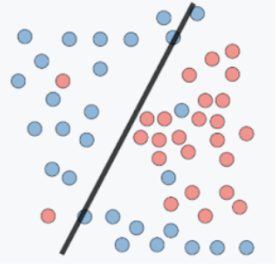
\includegraphics[width=4cm, height=2.5cm]{Figs/high-bias.png}
			\caption{High Variance, \href{https://tinyurl.com/2on8xr4o}{Source}}
			\label{fig:high-bias}
		\end{figure}
		
		\item The main options to fix this problem:
		
		\begin{itemize}
			\item Selecting a more powerful model, with more parameters
			\item Feeding better features to the learning algorithm (feature engineering)
			\item Reducing the constraints on the model (e.g., reducing the regularization hyperparameter)
		\end{itemize}
		
	\end{itemize}	
	
}
%%%%%%%%%%%%%%%%%%%%%%%%%%%%%%%%%%%%%%%%%%%%%%%%%%%%%%%%%%%%%%%%%%%%%%%%
\frame{\frametitle{Overfitting}
		
\begin{itemize}
    \item \tc{keywords}{Overfitting}means the model works well on training data, but it doesn't generalize well.
    
    \medskip
    \item Overfitting occurs when there is too much complexity in the model in comparison to the amount and noise in the training data.
    
    \begin{figure}
    	\centering
    	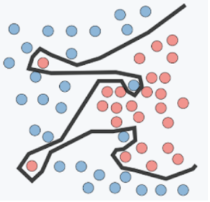
\includegraphics[width=4cm, height=2.5cm]{Figs/high-variance.png}
    	\caption{High Variance, \href{https://tinyurl.com/2on8xr4o}{Source}}
    	\label{fig:high-variance}
    \end{figure}
    
    \item Three practical solutions:
    \begin{itemize}
    	\item Simplify the model by selecting one with fewer parameters, reducing the number of attributes in the training
    	data, or constraining the model.
    	\item Gather more training data.
    	\item Reduce the noise in the training data.
    	
    \end{itemize}
    
\end{itemize}	
	
}

%%%%%%%%%%%%%%%%%%%%%%%%%%%%%%%%%%%%%%%%%%%%%%%%%%%%%%%%%%%%%%%%%%%%%%%%%%%
\frame{\frametitle{Overview}
	
	\begin{figure}
		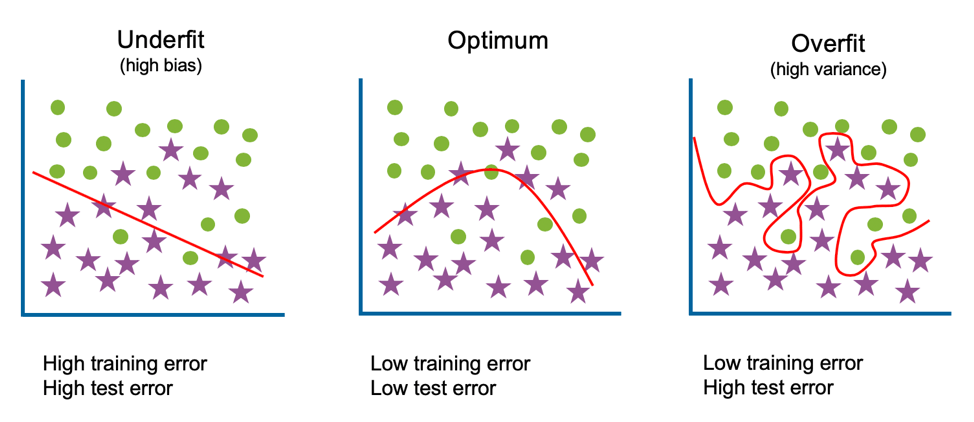
\includegraphics[width=12cm, height=5cm]{Figs/model-over-fitting.png}
		\caption{Overfitting vs Underfitting, \href{https://tinyurl.com/2n4kj86u}{Source}}
	\end{figure}

}


%%%%%%%%%%%%%%%%%%%%%%%%%%%%%%%%%%%%%%%%%%%%%%%%%%%%%%%%%%%%%%%%%%%%%%%%%%%
\frame{\frametitle{Overview}
	
	\begin{figure}
		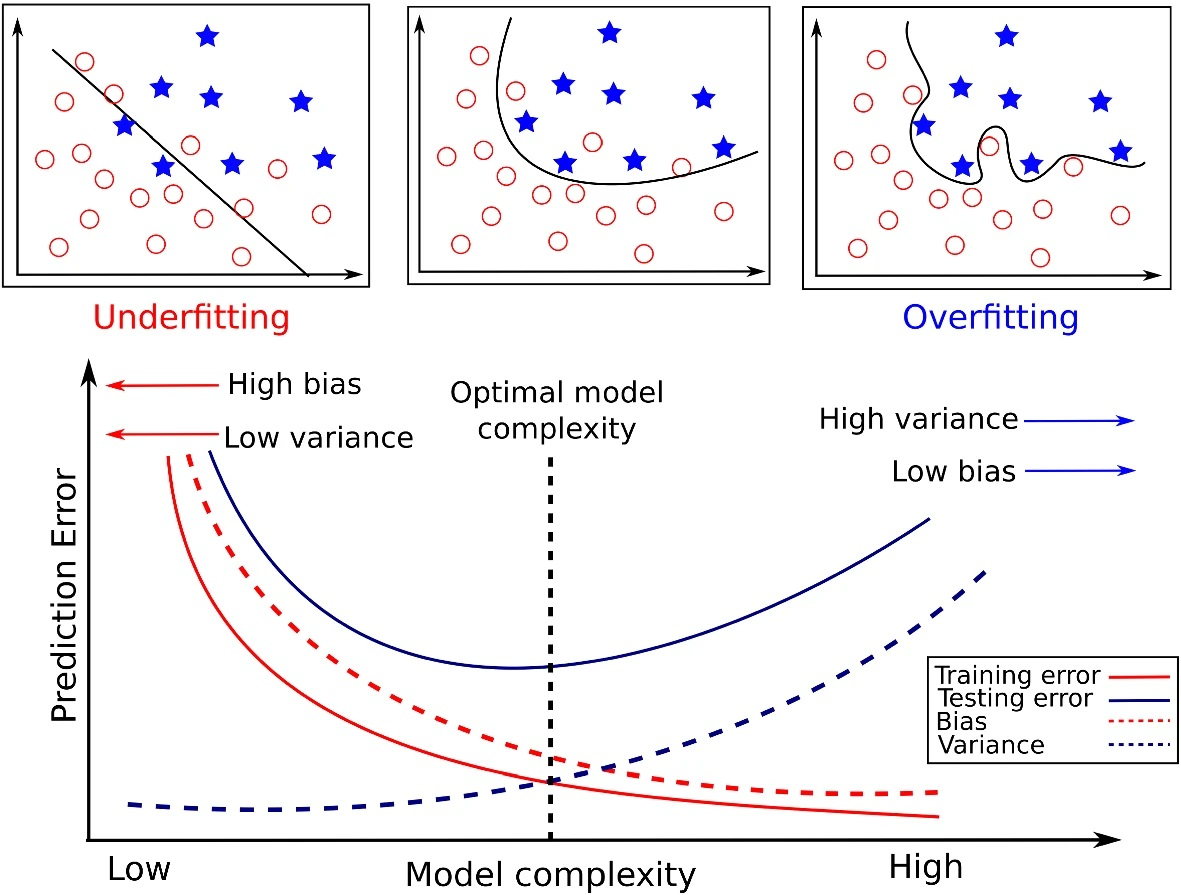
\includegraphics[width=8cm, height=6cm]{Figs/bias_vs_variance.jpg}
		\caption{Overfitting vs Underfitting, \href{https://tinyurl.com/2flpkzlm}{Source}}
	\end{figure}
	
}
%%%%%%%%%%%%%%%%%%%%
\frametitle{Final Notes}
\centering
\vspace{50 pt}
\textbf{Thank You!}
\vspace{50pt}

\textbf{Any Question?}
%%%%%%%%%%%%%%%%%%%%%%%%%%%%%%%%%%%%%%%%%%
\end{document}